% Options for packages loaded elsewhere
\PassOptionsToPackage{unicode}{hyperref}
\PassOptionsToPackage{hyphens}{url}
%
\documentclass[
]{book}
\usepackage{amsmath,amssymb}
\usepackage{lmodern}
\usepackage{iftex}
\ifPDFTeX
  \usepackage[T1]{fontenc}
  \usepackage[utf8]{inputenc}
  \usepackage{textcomp} % provide euro and other symbols
\else % if luatex or xetex
  \usepackage{unicode-math}
  \defaultfontfeatures{Scale=MatchLowercase}
  \defaultfontfeatures[\rmfamily]{Ligatures=TeX,Scale=1}
\fi
% Use upquote if available, for straight quotes in verbatim environments
\IfFileExists{upquote.sty}{\usepackage{upquote}}{}
\IfFileExists{microtype.sty}{% use microtype if available
  \usepackage[]{microtype}
  \UseMicrotypeSet[protrusion]{basicmath} % disable protrusion for tt fonts
}{}
\makeatletter
\@ifundefined{KOMAClassName}{% if non-KOMA class
  \IfFileExists{parskip.sty}{%
    \usepackage{parskip}
  }{% else
    \setlength{\parindent}{0pt}
    \setlength{\parskip}{6pt plus 2pt minus 1pt}}
}{% if KOMA class
  \KOMAoptions{parskip=half}}
\makeatother
\usepackage{xcolor}
\usepackage{color}
\usepackage{fancyvrb}
\newcommand{\VerbBar}{|}
\newcommand{\VERB}{\Verb[commandchars=\\\{\}]}
\DefineVerbatimEnvironment{Highlighting}{Verbatim}{commandchars=\\\{\}}
% Add ',fontsize=\small' for more characters per line
\usepackage{framed}
\definecolor{shadecolor}{RGB}{248,248,248}
\newenvironment{Shaded}{\begin{snugshade}}{\end{snugshade}}
\newcommand{\AlertTok}[1]{\textcolor[rgb]{0.94,0.16,0.16}{#1}}
\newcommand{\AnnotationTok}[1]{\textcolor[rgb]{0.56,0.35,0.01}{\textbf{\textit{#1}}}}
\newcommand{\AttributeTok}[1]{\textcolor[rgb]{0.77,0.63,0.00}{#1}}
\newcommand{\BaseNTok}[1]{\textcolor[rgb]{0.00,0.00,0.81}{#1}}
\newcommand{\BuiltInTok}[1]{#1}
\newcommand{\CharTok}[1]{\textcolor[rgb]{0.31,0.60,0.02}{#1}}
\newcommand{\CommentTok}[1]{\textcolor[rgb]{0.56,0.35,0.01}{\textit{#1}}}
\newcommand{\CommentVarTok}[1]{\textcolor[rgb]{0.56,0.35,0.01}{\textbf{\textit{#1}}}}
\newcommand{\ConstantTok}[1]{\textcolor[rgb]{0.00,0.00,0.00}{#1}}
\newcommand{\ControlFlowTok}[1]{\textcolor[rgb]{0.13,0.29,0.53}{\textbf{#1}}}
\newcommand{\DataTypeTok}[1]{\textcolor[rgb]{0.13,0.29,0.53}{#1}}
\newcommand{\DecValTok}[1]{\textcolor[rgb]{0.00,0.00,0.81}{#1}}
\newcommand{\DocumentationTok}[1]{\textcolor[rgb]{0.56,0.35,0.01}{\textbf{\textit{#1}}}}
\newcommand{\ErrorTok}[1]{\textcolor[rgb]{0.64,0.00,0.00}{\textbf{#1}}}
\newcommand{\ExtensionTok}[1]{#1}
\newcommand{\FloatTok}[1]{\textcolor[rgb]{0.00,0.00,0.81}{#1}}
\newcommand{\FunctionTok}[1]{\textcolor[rgb]{0.00,0.00,0.00}{#1}}
\newcommand{\ImportTok}[1]{#1}
\newcommand{\InformationTok}[1]{\textcolor[rgb]{0.56,0.35,0.01}{\textbf{\textit{#1}}}}
\newcommand{\KeywordTok}[1]{\textcolor[rgb]{0.13,0.29,0.53}{\textbf{#1}}}
\newcommand{\NormalTok}[1]{#1}
\newcommand{\OperatorTok}[1]{\textcolor[rgb]{0.81,0.36,0.00}{\textbf{#1}}}
\newcommand{\OtherTok}[1]{\textcolor[rgb]{0.56,0.35,0.01}{#1}}
\newcommand{\PreprocessorTok}[1]{\textcolor[rgb]{0.56,0.35,0.01}{\textit{#1}}}
\newcommand{\RegionMarkerTok}[1]{#1}
\newcommand{\SpecialCharTok}[1]{\textcolor[rgb]{0.00,0.00,0.00}{#1}}
\newcommand{\SpecialStringTok}[1]{\textcolor[rgb]{0.31,0.60,0.02}{#1}}
\newcommand{\StringTok}[1]{\textcolor[rgb]{0.31,0.60,0.02}{#1}}
\newcommand{\VariableTok}[1]{\textcolor[rgb]{0.00,0.00,0.00}{#1}}
\newcommand{\VerbatimStringTok}[1]{\textcolor[rgb]{0.31,0.60,0.02}{#1}}
\newcommand{\WarningTok}[1]{\textcolor[rgb]{0.56,0.35,0.01}{\textbf{\textit{#1}}}}
\usepackage{longtable,booktabs,array}
\usepackage{calc} % for calculating minipage widths
% Correct order of tables after \paragraph or \subparagraph
\usepackage{etoolbox}
\makeatletter
\patchcmd\longtable{\par}{\if@noskipsec\mbox{}\fi\par}{}{}
\makeatother
% Allow footnotes in longtable head/foot
\IfFileExists{footnotehyper.sty}{\usepackage{footnotehyper}}{\usepackage{footnote}}
\makesavenoteenv{longtable}
\usepackage{graphicx}
\makeatletter
\def\maxwidth{\ifdim\Gin@nat@width>\linewidth\linewidth\else\Gin@nat@width\fi}
\def\maxheight{\ifdim\Gin@nat@height>\textheight\textheight\else\Gin@nat@height\fi}
\makeatother
% Scale images if necessary, so that they will not overflow the page
% margins by default, and it is still possible to overwrite the defaults
% using explicit options in \includegraphics[width, height, ...]{}
\setkeys{Gin}{width=\maxwidth,height=\maxheight,keepaspectratio}
% Set default figure placement to htbp
\makeatletter
\def\fps@figure{htbp}
\makeatother
\setlength{\emergencystretch}{3em} % prevent overfull lines
\providecommand{\tightlist}{%
  \setlength{\itemsep}{0pt}\setlength{\parskip}{0pt}}
\setcounter{secnumdepth}{5}
\usepackage{booktabs}
\ifLuaTeX
  \usepackage{selnolig}  % disable illegal ligatures
\fi
\usepackage[]{natbib}
\bibliographystyle{plainnat}
\IfFileExists{bookmark.sty}{\usepackage{bookmark}}{\usepackage{hyperref}}
\IfFileExists{xurl.sty}{\usepackage{xurl}}{} % add URL line breaks if available
\urlstyle{same} % disable monospaced font for URLs
\hypersetup{
  pdftitle={Myocarditis Redcap wiki},
  pdfauthor={Charles Dolladille},
  hidelinks,
  pdfcreator={LaTeX via pandoc}}

\title{Myocarditis Redcap wiki}
\author{Charles Dolladille}
\date{2022-11-10}

\begin{document}
\maketitle

{
\setcounter{tocdepth}{1}
\tableofcontents
}
\hypertarget{about}{%
\chapter{About}\label{about}}

This is a reference document that describes the data structure and variables and the common data management schemes used for the analysis of the Myocarditis Redcap from Vanderbilt University.

\hypertarget{usage}{%
\section{Usage}\label{usage}}

This document is intended as a cheatsheet, for fast and easy reminder of data structure and variable names, and how to use them.

\hypertarget{target-users}{%
\section{Target users}\label{target-users}}

Cardiologist and data manager researchers from Drs Moslehi and Salem teams.

\hypertarget{intro}{%
\chapter{Introducing the database}\label{intro}}

This is a VERY brief introduction. The database was created in 2018, and gather more than 700 cases of immune checkpoint inhibitors associated cardiovascular adverse reactions (as of September 2022). Cases are reported from all around the world, and most of them are myocarditis cases.

\begin{quote}
October 2022 update. It was decided to remove all non-myocarditis cases from the base. Some cases were removed after a careful semi-automated review, which also tracked duplicates.
\end{quote}

If your not familiar with the Redcap data structure and how data can be exported, you should look at the Redcap Help \& FAQ. We will not deal with these concepts here.

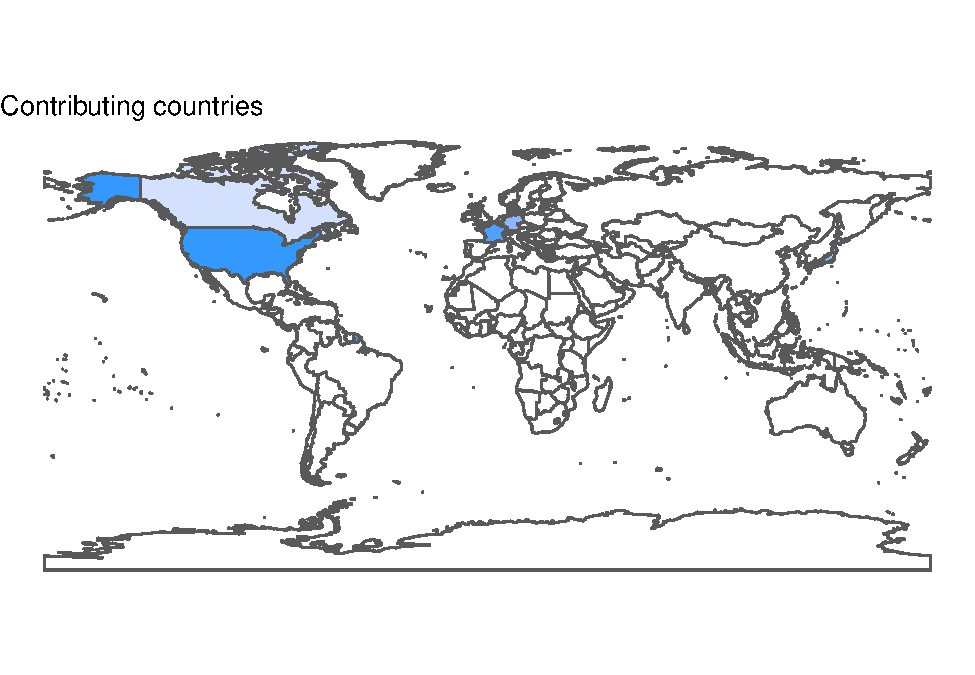
\includegraphics{_main_files/figure-latex/world_map-1.pdf}

\hypertarget{what-is-in-the-redcap}{%
\section{What is in the Redcap?}\label{what-is-in-the-redcap}}

In the Redcap you may find an extensive characterization of the cases, including clinical work-up and outcomes. These features are grouped according to time points (baseline, index date, follow-up\ldots) or critical exams (EKG, biopsy\ldots) that are called \textbf{instruments} in Redcap. Each instrument is described in a separate chapter in this document.

\hypertarget{variables-naming-rules}{%
\section{Variables naming rules}\label{variables-naming-rules}}

Variable names are attributed according to standardized rules as follow:

\begin{itemize}
\tightlist
\item
  A variable name always starts by the instrument identifier (e.g.~\texttt{p\_} for demographic data, see below \protect\hyperlink{data_structure}{Data structure}), with the exception of date \texttt{date\_}and time \texttt{ti\_} variables (see \protect\hyperlink{multi_instrument_var}{multi-instrument variables}).
\item
  In case an instrument is subdivided into multiple instruments, the instrument identifier is followed by the subinstrument identifier (e.g.~\texttt{ic\_ca} for index cardiotoxicity cancer treatment)
\item
  \protect\hyperlink{calc_manual_var}{Calculated vars} have the same name as manual vars, with an additional suffix \texttt{\_\_c}.
\item
  \protect\hyperlink{freetext_var}{Free text vars} have the same name as their branching logic displayer, with an additional suffix \texttt{\_\_ft}.
\item
  Descriptive vars have the same name as their branching logic displayer, with an additional suffix \texttt{\_\_desc}. Note that these vars do not contain any data and are not usually exported.
\item
  All variables names are lower case, with words separated by underscores (e.g.~you will not see upper case vars such as \texttt{AGE\_VAR}). This is also known as \texttt{snake\_case} format.
\item
  As much as possible, we use singular rather than plural in the names (e.g.~\texttt{antimetabolite} rather than \texttt{antimetabolites})
\item
  Variables with the \texttt{\_\_old} suffix are former versions that will be integrated in v3 of the database. They contain the same type of information, but often have different levels (e.g.~an additional ``missing'' level).
\end{itemize}

We translate here a general description of the variables. To get a precise definition of a variable, you will be more inspired looking at the Redcap's codebook.

\textbf{Please note} this document is NOT an exhaustive list of the variables in the redcap and is not intended to be.

\hypertarget{data_structure}{%
\section{Data structure}\label{data_structure}}

The Redcap instruments are:

\begin{longtable}[]{@{}
  >{\raggedright\arraybackslash}p{(\columnwidth - 4\tabcolsep) * \real{0.2034}}
  >{\raggedright\arraybackslash}p{(\columnwidth - 4\tabcolsep) * \real{0.0734}}
  >{\raggedright\arraybackslash}p{(\columnwidth - 4\tabcolsep) * \real{0.7232}}@{}}
\toprule()
\begin{minipage}[b]{\linewidth}\raggedright
Instrument
\end{minipage} & \begin{minipage}[b]{\linewidth}\raggedright
Identifier
\end{minipage} & \begin{minipage}[b]{\linewidth}\raggedright
Description
\end{minipage} \\
\midrule()
\endhead
\protect\hyperlink{admin}{Admin} & {[}ad{]} & Identify the reporting source, the reporter, with mailing contact information. \\
\protect\hyperlink{demo}{Demographics} & {[}p{]} & Patient demographics (age, sex\ldots), medical history (including cardiovascular history), and medications. \\
\protect\hyperlink{base_ekg}{Baseline EKG} & {[}be{]} & If any, description of a baseline Electrocardiogram (prior to cardiotoxicity). \\
\protect\hyperlink{previous_line}{Previous line} & {[}pl{]} & Features of prior anticancer treatments, including those of older cancers and the current cancer in prior lines of treatment. \\
\protect\hyperlink{current_line}{Current line} & {[}cl{]} & Features of the current line of anticancer treatment containing immunotherapy(ies).

Also, features of the current cancer (actively treated). \\
\protect\hyperlink{index_c}{Index cardiotoxicity} & {[}ic{]} & All clinical work-up of the patient when presenting for cardiotoxicity. This is the main instrument. \\
\protect\hyperlink{index_ekg}{Index EKG} & {[}ie{]} & It is an instrument by itself, as it gathers one or several EKGs, hence there is a large quantity of data here. \\
\protect\hyperlink{index_h}{Index hospitalization} & {[}ih{]} & Features that occurred during the hospitalization that followed cardiotoxicity diagnosis. \\
\protect\hyperlink{fup}{Follow-up} & {[}fu{]} & Long term outcomes. \\
\protect\hyperlink{biology}{Biology} & {[}b & All biological features (transversal instrument) \\
\bottomrule()
\end{longtable}

\hypertarget{multi-instrument-variables}{%
\section{Multi-instrument variables}\label{multi-instrument-variables}}

Sometime, an event can occur at different times. For example, a patient can experience death during its index hospitalization, or later in follow-up. To ensure a proper identification of events according to the research purpose, \protect\hyperlink{multi_instrument_var}{a separate chapter is dedicated to theses variables} including timings.

\hypertarget{root-variables}{%
\section{Root variables}\label{root-variables}}

When a question can have multiple non-exclusive answers, the Field Type in Redcap is ``checklist''.

For example: which alkylating agent(s) was(were) used?

\begin{itemize}
\item
  Cisplatin
\item
  Carboplatin
\end{itemize}

Suppose the dots are checkboxes and you may select either of them.

In this case, Redcap creates subvariables in the data extraction. If the variable name is \texttt{p\_pl\_alkylating\_agent}, then you will NOT find it in the extraction. You will have 2 subvariables named \texttt{p\_pl\_alkylating\_agent\_\_\_1} and \texttt{p\_pl\_alkylating\_agent\_\_\_2}.

\begin{quote}
Root variables are those variables that are splitted into multiple subvariables, i.e.~which have the Field Type argument ``checkbox''.
\end{quote}

You may want to merge back these variables together, to create a global variable: ``Has the patient been treated with any alkylating agent?''.

\hypertarget{admin}{%
\chapter{Admin}\label{admin}}

\begin{quote}
Admin variable identifier is {[}ad{]}
\end{quote}

It is the first chapter but actually, administrative variables are quite easy to use.

There is a few logical branching here. If you want to create a country-level variable, you will need to gather back several subvariables including \texttt{reporting\_region}, (USA are a stand alone in this variable) \texttt{european\_countries}, \texttt{african\_countries}, \texttt{asian\_countries}, \texttt{australia\_countries}. These variables are mutually exclusive (except for reporting\_region).

Useful when you want to draw the world map of contributing countries.

Please look at the \protect\hyperlink{contrib}{contributors and contributing centers} section for more details.

\hypertarget{demo}{%
\chapter{Demographics}\label{demo}}

\begin{quote}
Demographics variable identifier is {[}p{]} for patient
\end{quote}

\hypertarget{abbreviations}{%
\section{Abbreviations}\label{abbreviations}}

Here is a list of abbreviations used in several variables in the demo instrument.

\begin{longtable}[]{@{}
  >{\raggedright\arraybackslash}p{(\columnwidth - 2\tabcolsep) * \real{0.1280}}
  >{\raggedright\arraybackslash}p{(\columnwidth - 2\tabcolsep) * \real{0.8720}}@{}}
\toprule()
\begin{minipage}[b]{\linewidth}\raggedright
Abbreviation(s)
\end{minipage} & \begin{minipage}[b]{\linewidth}\raggedright
Feature
\end{minipage} \\
\midrule()
\endhead
\texttt{cancer\_hx}

\texttt{cx} & Cancer history: refers to prior cancer(s) the patient had in his/her life before the one actively treated with immune checkpoint inhibitors.

\texttt{cx1}, \texttt{2}, \texttt{3}\ldots{} Refer to features for specifics types of cancer (1 is Bladder cancer, 2 is Breast cancer, etc.) \\
\texttt{pl} & Previous line: this is a concept to refer to treatments received either for prior cancer(s) \textbf{or} \textbf{the current cancer} in previous lines

Obviously falls inbetween two instruments (demographics and current cancer) \\
\texttt{autoimmune\_hx}

\texttt{ai} & Auto-immune history: prior auto-immune disease \\
\texttt{organ\_transplant}

\texttt{ot} & Organ transplantation history \\
\bottomrule()
\end{longtable}

\hypertarget{calculated-variables}{%
\section{Calculated variables}\label{calculated-variables}}

You can check the difference between calculated and manual vars \protect\hyperlink{calc_manual_var}{here}.

\begin{longtable}[]{@{}ll@{}}
\toprule()
manual var & calculated var \\
\midrule()
\endhead
\texttt{p\_age} & \texttt{p\_age\_\_c} \\
\texttt{p\_bmi} & \texttt{p\_bmi\_\_c} \\
\bottomrule()
\end{longtable}

\hypertarget{derived-variables}{%
\section{Derived variables}\label{derived-variables}}

\hypertarget{categorical-body-mass-index-and-overweight-or-obese}{%
\subsection{Categorical Body Mass Index and overweight or obese}\label{categorical-body-mass-index-and-overweight-or-obese}}

For the latter, read as is patients BMI\textgreater25 or not?

\begin{Shaded}
\begin{Highlighting}[]
\NormalTok{p\_bmi\_cat }\OtherTok{=} \FunctionTok{expr}\NormalTok{(}
  \FunctionTok{case\_when}\NormalTok{(}
\NormalTok{      p\_bmi }\SpecialCharTok{\textless{}} \FloatTok{18.5} \SpecialCharTok{\textasciitilde{}} \StringTok{"underweight"}\NormalTok{,}
\NormalTok{      dplyr}\SpecialCharTok{::}\FunctionTok{between}\NormalTok{(p\_bmi, }\FloatTok{18.5}\NormalTok{, }\DecValTok{25}\NormalTok{) }\SpecialCharTok{\textasciitilde{}} \StringTok{"normal\_weight"}\NormalTok{,}
\NormalTok{      dplyr}\SpecialCharTok{::}\FunctionTok{between}\NormalTok{(p\_bmi, }\DecValTok{25}\NormalTok{, }\DecValTok{30}\NormalTok{) }\SpecialCharTok{\textasciitilde{}} \StringTok{"overweight"}\NormalTok{,}
\NormalTok{      p\_bmi }\SpecialCharTok{\textgreater{}} \DecValTok{30} \SpecialCharTok{\textasciitilde{}} \StringTok{"obese"}
\NormalTok{    ))}

\NormalTok{p\_overweight\_obese }\OtherTok{=} \FunctionTok{expr}\NormalTok{(}
  \FunctionTok{if\_else}\NormalTok{(}
\NormalTok{      p\_bmi }\SpecialCharTok{\textgreater{}} \DecValTok{25}\NormalTok{, }
      \DecValTok{1}\NormalTok{, }
      \DecValTok{0}
\NormalTok{    )}
\NormalTok{)}
\end{Highlighting}
\end{Shaded}

\hypertarget{cardiovascular-risk-factors}{%
\subsection{Cardiovascular risk factors}\label{cardiovascular-risk-factors}}

At least one traditional cardiovascular risk factor

\begin{Shaded}
\begin{Highlighting}[]
\NormalTok{p\_cv\_risk }\OtherTok{=} \FunctionTok{expr}\NormalTok{(}
  \FunctionTok{pmax}\NormalTok{(}
\NormalTok{      p\_lipid\_chol,}
\NormalTok{      p\_tobacco\_anytime,}
\NormalTok{      p\_diabetes2,}
\NormalTok{      p\_hypertension,}
      \AttributeTok{na.rm =} \ConstantTok{TRUE}
\NormalTok{    )}
\NormalTok{  )}
\end{Highlighting}
\end{Shaded}

\hypertarget{medications}{%
\section{Medications}\label{medications}}

There is always an ambiguity with checkboxes: if nothing is checked, you can't tell if the answer is negative to your question, or if the data is missing.

For example, if you have two checkboxes for medications

\begin{itemize}
\item
  Beta-blockers
\item
  Aspirin
\end{itemize}

And say the first is checked and the second is not. In this case, its easy to say the patient is taking betablockers, but what about aspirin? Maybe the patient is not taking aspirin, or maybe data is missing and the user did not checked the box. This could be the case if a patient addressed to the hospital forgets to bring his/her prescription and do not remember precisely the name of the medications. On the other hand, you may often retrieve the complete list by calling the pharmacist or if a related finally brings the prescription during the hospital stay.

\begin{quote}
It is assumed that medication list is complete (no missing data) if the \texttt{p\_meds\_any} variable is checked.
\end{quote}

\hypertarget{current_line}{%
\chapter{Current line}\label{current_line}}

\begin{quote}
Current line identifier is {[}cl{]}
\end{quote}

\hypertarget{definition}{%
\section{Definition}\label{definition}}

The current line is the most recently administered cure of anticancer drugs that contains immune checkpoint inhibitors. It can be ongoing at the time of index cardiotoxicity, or may have been interrupted.

\hypertarget{abbreviations-1}{%
\section{Abbreviations}\label{abbreviations-1}}

Abbreviations for immune checkpoint inhibitor drugs and classes are the same as in \protect\hyperlink{previous_line_ab_table}{the previous line instrument}.

Here is a list of abbreviations used in several variables in the current line instrument.

\begin{longtable}[]{@{}ll@{}}
\toprule()
Abbreviation(s) & Feature \\
\midrule()
\endhead
\texttt{1stdrug} & Refers to the 1st infusion of the drug \\
\texttt{lastdrug} & Refers to the last infusion of the drug \\
\bottomrule()
\end{longtable}

\hypertarget{index_c}{%
\chapter{Index cardiotoxicity}\label{index_c}}

\begin{quote}
Index cardiotoxicity identifier is {[}ic{]}
\end{quote}

There is a little ambiguity here: index cardiotoxicity refers both to the date of cardiotoxicity diagnosis AND date of hospital admission (if any) for this cardiotoxicity.

\hypertarget{abbreviations-2}{%
\section{Abbreviations}\label{abbreviations-2}}

\begin{longtable}[]{@{}
  >{\raggedright\arraybackslash}p{(\columnwidth - 2\tabcolsep) * \real{0.1429}}
  >{\raggedright\arraybackslash}p{(\columnwidth - 2\tabcolsep) * \real{0.8571}}@{}}
\toprule()
\begin{minipage}[b]{\linewidth}\raggedright
Abbreviation(s)
\end{minipage} & \begin{minipage}[b]{\linewidth}\raggedright
Feature
\end{minipage} \\
\midrule()
\endhead
Clinical work-up & \\
\texttt{sy} & Symptoms \\
\texttt{ctx} & Cardiotoxicity (used for the description of timings between a ctx symptoms \texttt{ctx\ sy} and index date, and grading). \\
\texttt{pe} & Physical examination features \\
\texttt{irae} & Features of non-cardiac immune related adverse events at the index date \\
\texttt{hyper,\ hypo,\ aiha,\ attp,\ hus,\ aa,\ id,\ bd,\ scar} & For iraes subclasses, small adds to refer to the correct subclass (hyperthyroidism, hypothyroidism, auto-immune hemolytic anemia, acquired thrombotic thrombocytopenic purpura, hemolytic and uremic syndrome, aplastic anemia, inflammatory dermatitis, bullous dermatosis, severe cutaneous adverse reaction) \\
Exams & \\
\texttt{bx} & Biopsy features (muscular, cardiac, other) \\
\texttt{lhc} & Left Heart Catheterization \\
Treatment section

\texttt{tx} & \\
immsup & Immunosuppressant \\
& 4-character abbreviation for immunosuppressants \\
\texttt{ivig}

\texttt{plas}

\texttt{tacy}

\texttt{myco}

\texttt{othr}

\texttt{athg}

\texttt{infl}

\texttt{abab}

\texttt{mtor}

\texttt{cycl}

\texttt{azat}

\texttt{ritu} & Intravenous Immunoglobulin

Plasmapheresis (PLEX)

Tacrolimus or cyclosporin

Mycophenolate mofetil

Other immunosuppressant

ATG / thymoglobulin

Infliximab or other anti-TNFalpha

Abatacept or belatacept

mTOR inhibitors (temsirolimus, everolimus, sirolimus)

Cyclophosphamide

Azathioprine

Rituximab \\
\texttt{ms} & Mechanical support \\
\texttt{aa} & Anti-arrhythmic drugs or devices \\
\bottomrule()
\end{longtable}

\hypertarget{biological-features}{%
\section{Biological features}\label{biological-features}}

Most normal values of biological parameters are different from one lab to another. Also, users may report bio vars according to different scales.

Examples: troponin upper limit of normal may range from \textasciitilde{} 0.01 to \textasciitilde{} 50. Complete blood count can be reported in G/L or 10\^{}-3/µL (even if the var field asked for reporting with one of them).

It is advised to express biological parameters according to their normal value range if known, or to contrast them into ratios that get rid of the unit (example: neutrophil to lymphocyte ratio)

\hypertarget{index_h}{%
\chapter{Index hospitalization}\label{index_h}}

\begin{quote}
Index hospitalization identifier is {[}ih{]}
\end{quote}

Features occurring early after index cardiotoxicity. It encompasses repeated EKG, echos, and complications.

\hypertarget{abbreviations-3}{%
\section{Abbreviations}\label{abbreviations-3}}

\begin{longtable}[]{@{}
  >{\raggedright\arraybackslash}p{(\columnwidth - 2\tabcolsep) * \real{0.1208}}
  >{\raggedright\arraybackslash}p{(\columnwidth - 2\tabcolsep) * \real{0.8792}}@{}}
\toprule()
\begin{minipage}[b]{\linewidth}\raggedright
Abbreviation(s)
\end{minipage} & \begin{minipage}[b]{\linewidth}\raggedright
Feature
\end{minipage} \\
\midrule()
\endhead
\texttt{wstecho} & The worst echocardiographia (the one with the lowest Left Ventricular Ejection Fraction) \\
\texttt{wstmri} & The worst Cardiac Magnetic Resonance Imaging (note that it might not be the most demonstrative MRI, according to the definition) \\
Outcome section

\texttt{ou} & \\
\texttt{o1,\ o2} & Organ 1, 2, 3, affected by sepsis \\
\texttt{rf} & Respiratory failure \\
\bottomrule()
\end{longtable}

\hypertarget{previous_line}{%
\chapter{Previous line}\label{previous_line}}

\begin{quote}
Previous line identifier is {[}pl{]}
\end{quote}

\hypertarget{definition-1}{%
\section{Definition}\label{definition-1}}

Instrument previous line refers to any anticancer treatment received, either for a prior cancer \textbf{or for the current cancer}, before the current line.

The \protect\hyperlink{current_line}{current line} is the most recently administered one that contains immune checkpoint inhibitors. It can be ongoing at the time of index cardiotoxicity, or may have been interrupted.

\hypertarget{previous_line_ab_table}{%
\section{Abbreviations}\label{previous_line_ab_table}}

Here is a list of abbreviations used in several variables in the demo instrument.

\begin{longtable}[]{@{}
  >{\raggedright\arraybackslash}p{(\columnwidth - 2\tabcolsep) * \real{0.1104}}
  >{\raggedright\arraybackslash}p{(\columnwidth - 2\tabcolsep) * \real{0.8896}}@{}}
\toprule()
\begin{minipage}[b]{\linewidth}\raggedright
Abbreviation(s)
\end{minipage} & \begin{minipage}[b]{\linewidth}\raggedright
Feature
\end{minipage} \\
\midrule()
\endhead
\texttt{atez}

\texttt{avel}

\texttt{cemi}

\texttt{durv}

\texttt{nivo}

\texttt{ipil}

\texttt{pemb}

\texttt{trem} & Standardized \textbf{4-character} abbreviations of immune checkpoint inhibitors

Atezolizumab, avelumab, cemiplimab, durvalumab, nivolumab, ipilimumab, pembrolizumab, tremelimumab \\
\texttt{pd1}

\texttt{pdl1}

\texttt{ctla4} & When drug name is not know, standardized abbreviations related to ICI class.

Anti-PD1, anti-PD-L1, anti-CTLA4

Also \texttt{pd1\_other}, \texttt{pdl1\_other}, and \texttt{ctla4\_other} to refer to an ICI from a class that is not in the aforementioned list (e.g.~a new anti-PD1) \\
\bottomrule()
\end{longtable}

\hypertarget{use_case}{%
\chapter{Common use cases}\label{use_case}}

\hypertarget{calc_manual_var}{%
\section{Calculated versus manual vars}\label{calc_manual_var}}

Many numeric variables can be entered in two ways:

\begin{itemize}
\item
  \textbf{calculated var:} The user provides dates (e.g., date of birth,
  date of index cardiotoxicity), and the variable is automatically
  calculated from these dates (e.g.~age as the difference between
  index cardiotoxicity date and date of birth).
\item
  \textbf{manual var:} The user could not provide dates, but had a free
  text field to input the value.
\end{itemize}

As a result, 2 variables contain the same data. They are not mutually
exclusive, which means an observation can have a value for the 2
variables (e.g.~the user provided both dates, which allows for automated
computation in the calculated var, and also entered age in the manual
var free text variable). There has to be a rule of thumb to choose which
variable is to be used in the analysis. Here is ours:

\begin{quote}
Calculated vars are preferred over manual vars
\end{quote}

This means that, for a single case:

\begin{itemize}
\item
  If the calculated var is available, it will be retained.
\item
  Else, if the manual var is available, it will be retained.
\item
  Else, if none are available, the value is missing.
\end{itemize}

Here is an implementation of this simple logic into an R function

\begin{Shaded}
\begin{Highlighting}[]
\NormalTok{numvar\_uni }\OtherTok{\textless{}{-}} \CommentTok{\# Numeric variables unifier}
  \ControlFlowTok{function}\NormalTok{( }\CommentTok{\# used to organize data entered from 2 variables, currently its a prioritization}
\NormalTok{    var1, }\CommentTok{\# a quasi quoted name of column from data. Usually, one is the calculated var, one is the manual var, var1 will be prioritize over var2}
\NormalTok{    var2 }\CommentTok{\# also a quasi quoted name}
    \CommentTok{\# underlying data.frame data argument is omitted}
\NormalTok{  )\{}
\NormalTok{    var1 }\OtherTok{\textless{}{-}}\NormalTok{ rlang}\SpecialCharTok{::}\FunctionTok{enexpr}\NormalTok{(var1)}
\NormalTok{    var2 }\OtherTok{\textless{}{-}}\NormalTok{ rlang}\SpecialCharTok{::}\FunctionTok{enexpr}\NormalTok{(var2)}
    
\NormalTok{    ex }\OtherTok{\textless{}{-}}\NormalTok{ rlang}\SpecialCharTok{::}\FunctionTok{expr}\NormalTok{(dplyr}\SpecialCharTok{::}\FunctionTok{case\_when}\NormalTok{(}
      \SpecialCharTok{!}\FunctionTok{is.na}\NormalTok{(}\SpecialCharTok{!!}\NormalTok{var1) }\SpecialCharTok{\textasciitilde{}} \FunctionTok{as.numeric}\NormalTok{(}\SpecialCharTok{!!}\NormalTok{var1),}
      \SpecialCharTok{!}\FunctionTok{is.na}\NormalTok{(}\SpecialCharTok{!!}\NormalTok{var2) }\SpecialCharTok{\textasciitilde{}} \FunctionTok{as.numeric}\NormalTok{(}\SpecialCharTok{!!}\NormalTok{var2),}
      \ConstantTok{TRUE} \SpecialCharTok{\textasciitilde{}} \ConstantTok{NA\_real\_}
\NormalTok{    ))}
    
\NormalTok{    ex}
\NormalTok{  \}}
\end{Highlighting}
\end{Shaded}

\hypertarget{calculated-and-manual-vars-identifiers}{%
\section{Calculated and manual vars identifiers}\label{calculated-and-manual-vars-identifiers}}

\begin{quote}
For a manual var, the associated calculated var has the \textbf{\texttt{\_\_c}}
suffix.
\end{quote}

Example:

\begin{longtable}[]{@{}ll@{}}
\toprule()
manual var & calculated var \\
\midrule()
\endhead
\texttt{p\_age} (patient age, from instrument admin) & \texttt{p\_age\_\_c} \\
\bottomrule()
\end{longtable}

\hypertarget{freetext_var}{%
\section{Free text variables}\label{freetext_var}}

Users are often provided additional fields in the case their patient
falls out of the checkboxes. For example, a patient may have experienced
an auto-immune disease that is not listed in the \texttt{p\_ai\_} vars.

In this case, the user can check the \texttt{p\_ai\_other} box. When this box is
checked, the \texttt{p\_ai\_other\_\_ft} variable is displayed. It is a free text
field where the user can input additional data (e.g.~Bullous
pemphigoid).

\begin{quote}
Free text vars have the same name as the branching logic displayer,
with a \texttt{\_\_ft} suffix.
\end{quote}

At the moment, data from free text variables is not used to compute
additional variables for 2 main reasons:

\begin{itemize}
\item
  There are few data in these vars
\item
  Data quality checking requires additional time consuming ressources
  that cannot be applied to a general framework
\end{itemize}

\begin{quote}
We recommend you use free text variables only if their data closely
match your research question.
\end{quote}

\hypertarget{sex}{%
\section{Sex}\label{sex}}

At this stage, it is a binary variable with value

\begin{itemize}
\item
  1 for man
\item
  2 for woman
\end{itemize}

It is usually easier to use a variable named ``man'' or ``woman'', built
from the sex variable, to remember how to interprate model results.

\hypertarget{multi_instrument_var}{%
\chapter{Multi-instrument variables}\label{multi_instrument_var}}

\hypertarget{date-and-time-variables}{%
\section{Date and time variables}\label{date-and-time-variables}}

As dates and times are used across instruments to capture delays between an event and another (e.g.~between index cardiotoxicity and death), there are attributed a specific naming scheme:

\begin{itemize}
\item
  They do not start by the instrument identifier
\item
  They have their own identifier \texttt{date} for dates and \texttt{ti} for times.
\item
  Time variables always have 3 components:

  \begin{itemize}
  \item
    The \texttt{ti} identifier
  \item
    The first event identifier
  \item
    The second event identifier
  \end{itemize}
\end{itemize}

There is an exception to this naming rule: time between 2 cures of ICI (either previous line or current line), which has the long suffix \texttt{regimen\_freq}.

For example, time between index cardiotoxicity and death is \texttt{ti\_ic\_death}. An event identifier can have a middle \texttt{\_} if its very long (e.g.~\texttt{cl1stctla4\_other}~for current line first dose of an unspecified anti-CTLA4, although this is quite a rare case.

\begin{quote}
Time variables represent \textbf{delays} between two dates.
\end{quote}

Of note, times can be expressed in days, weeks or years.

\begin{longtable}[]{@{}
  >{\raggedright\arraybackslash}p{(\columnwidth - 6\tabcolsep) * \real{0.2252}}
  >{\raggedright\arraybackslash}p{(\columnwidth - 6\tabcolsep) * \real{0.1441}}
  >{\raggedright\arraybackslash}p{(\columnwidth - 6\tabcolsep) * \real{0.1081}}
  >{\raggedright\arraybackslash}p{(\columnwidth - 6\tabcolsep) * \real{0.5225}}@{}}
\toprule()
\begin{minipage}[b]{\linewidth}\raggedright
var
\end{minipage} & \begin{minipage}[b]{\linewidth}\raggedright
instrument
\end{minipage} & \begin{minipage}[b]{\linewidth}\raggedright
unit
\end{minipage} & \begin{minipage}[b]{\linewidth}\raggedright
quick desc
\end{minipage} \\
\midrule()
\endhead
\texttt{ti\_tobaccoquit\_ic} & demo & years & From tobacco quitting to IC \\
\texttt{ti\_otx\_ic} & demo & years & From organ transplant x to IC \\
\texttt{ti\_plicistop\_ic} & demo & days & From previous line ICI stop (end of regimen) to IC \\
\texttt{pl\_drug\_regimen\_freq} & previous\_line & weeks & From one cure to another, during an ICI therapy regimen \\
\texttt{ti\_ic\_1ststeroid} & ic & days & From IC to first dose of steroids \\
\texttt{ti\_cl1stnivo\_ic} & cl & days & From current line ICI-drug 1st infusion to IC \\
\texttt{ti\_ic\_ihdischarge} & ih & days & Length of hospital stay \\
& & & \\
& & & \\
& & & \\
& & & \\
\bottomrule()
\end{longtable}

\hypertarget{time-to-cardiotoxicity-onset-from-immune-checkpoint-inhibitor-introduction}{%
\section{Time to cardiotoxicity onset from immune checkpoint inhibitor introduction}\label{time-to-cardiotoxicity-onset-from-immune-checkpoint-inhibitor-introduction}}

As the title suggests, the idea is to collect the time to onset between the \textbf{first dose} of immune checkpoint inhibitor received \textbf{during the current cycle} and the occurrence of cardiotoxicity.

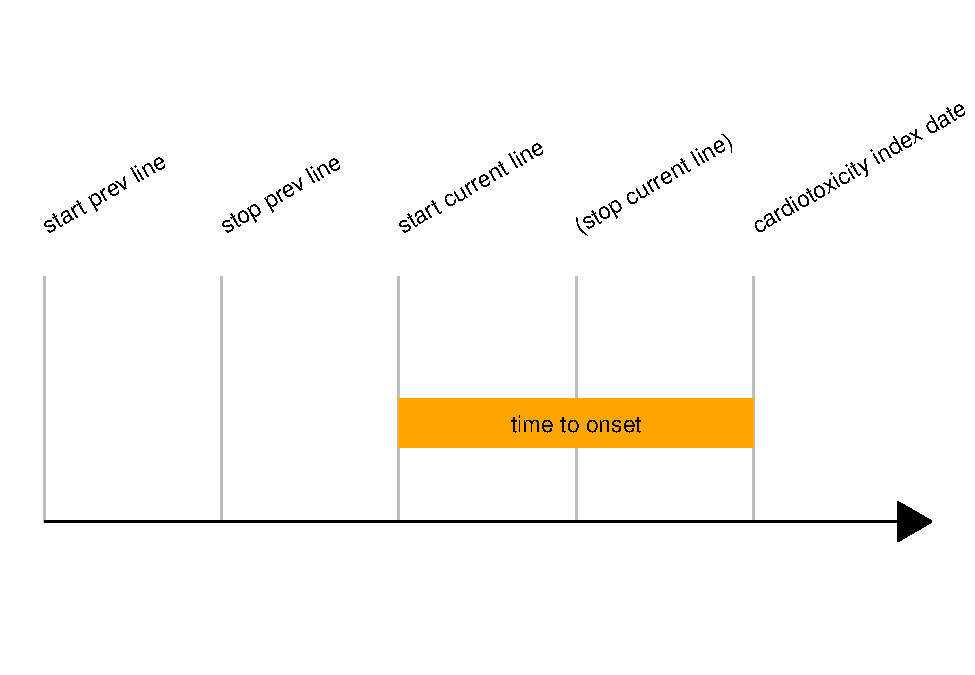
\includegraphics{_main_files/figure-latex/unnamed-chunk-5-1.pdf}

This data is stored at the immune checkpoint inhibitor level, e.g., a patient who received nivolumab will have this data stored in a nivolumab specific variable. The structure for this data is

\begin{longtable}[]{@{}
  >{\raggedright\arraybackslash}p{(\columnwidth - 4\tabcolsep) * \real{0.1190}}
  >{\raggedright\arraybackslash}p{(\columnwidth - 4\tabcolsep) * \real{0.1429}}
  >{\raggedright\arraybackslash}p{(\columnwidth - 4\tabcolsep) * \real{0.7381}}@{}}
\toprule()
\begin{minipage}[b]{\linewidth}\raggedright
Current
\end{minipage} & \begin{minipage}[b]{\linewidth}\raggedright
Target
\end{minipage} & \begin{minipage}[b]{\linewidth}\raggedright
Description
\end{minipage} \\
\midrule()
\endhead
\texttt{start\_days\_drug} & \texttt{ti\_icistart\_ic\_drug} & It is a \textbf{delay}, in days. Drug name is abbreviated here in the current naming (e.g.~nivo for nivolumab). Sometimes, the drug name is wrong (see below)

Could be : time variable (ti\_) from (ici\_start) to index cardiotoxicity (ic), for drug (drug complete name) \\
\texttt{start\_days\_drugx} & \texttt{ti\_icistart\_ic\_drug\_\_calc} & Same but computed from dates (when available). Mind the ``x'' at the end of the name

Could be: same but with a standardized suffix indicating a calculation \\
\texttt{first\_doses\_drug\_mce} & & Drug name is complete here. It is an old variable which has now the \textbackslash@ HIDDEN status, and is similar to start\_days\_drugx \\
\bottomrule()
\end{longtable}

To capture this time to onset, you have to check every possibilities for a patient, e.g.~you must check for all immune checkpoint inhibitor level time variables and choose which of these 3 variables you keep first, if ever more than one is available. This gives a quite heavy piece of code

\begin{Shaded}
\begin{Highlighting}[]
\NormalTok{ti\_icistart\_ic }\OtherTok{=} \FunctionTok{expr}\NormalTok{(}\FunctionTok{pmax}\NormalTok{( }\CommentTok{\# pmax here: maximum delay (in the case multiple ICI were prescribed sequentially)}
   \FunctionTok{eval}\NormalTok{(}\FunctionTok{tto\_uni\_3v}\NormalTok{(start\_days\_nivo,}
\NormalTok{                 start\_days\_nivox,}
\NormalTok{                 first\_doses\_nivolumab\_mce)), }\CommentTok{\# identical to start\_days\_nivox but it is @HIDDEN}
   \FunctionTok{eval}\NormalTok{(}\FunctionTok{tto\_uni\_3v}\NormalTok{(start\_days\_pem,}
\NormalTok{                 start\_days\_pemx,}
\NormalTok{                 first\_doses\_pembrolizumab\_mce)), }\CommentTok{\# @HIDDEN}
   \FunctionTok{eval}\NormalTok{(}\FunctionTok{tto\_uni\_3v}\NormalTok{(start\_days\_pem\_2, }\CommentTok{\# Other Anti{-}PD1 regimen}
\NormalTok{                 start\_days\_pem\_2x,}
\NormalTok{                 first\_doses\_pembrolizumab\_mce\_2)),}\CommentTok{\# @HIDDEN}
   \FunctionTok{eval}\NormalTok{(}\FunctionTok{tto\_uni\_3v}\NormalTok{(start\_days\_pem\_3, }\CommentTok{\# Cemiplimab }
\NormalTok{                 start\_days\_pem\_3x,}
\NormalTok{                 first\_doses\_pembrolizumab\_mce\_3)),}
   \FunctionTok{eval}\NormalTok{(}\FunctionTok{tto\_uni\_3v}\NormalTok{(start\_days\_atez,}
\NormalTok{                 start\_days\_atezx,}
\NormalTok{                 first\_doses\_atezolizumab\_mce)),}
   \FunctionTok{eval}\NormalTok{(}\FunctionTok{tto\_uni\_3v}\NormalTok{(start\_days\_ave,}
\NormalTok{                 start\_days\_avex,}
\NormalTok{                 first\_doses\_avelumab\_mce)),}
   \FunctionTok{eval}\NormalTok{(}\FunctionTok{tto\_uni\_3v}\NormalTok{(start\_days\_durv,}
\NormalTok{                 start\_days\_durvx,}
\NormalTok{                 first\_doses\_durvalumab\_mce)),}
   \FunctionTok{eval}\NormalTok{(}\FunctionTok{tto\_uni\_3v}\NormalTok{(start\_days\_durv\_3,}\CommentTok{\# Ohter Anti{-}PDL1}
\NormalTok{                 start\_days\_durv\_3x,}
\NormalTok{                 first\_doses\_durvalumab\_mce\_3)),}
   \FunctionTok{eval}\NormalTok{(}\FunctionTok{tto\_uni\_3v}\NormalTok{(start\_days\_ipi,}
\NormalTok{                 start\_days\_ipix,}
\NormalTok{                 first\_doses\_ipilimumab\_mce)),}
   \FunctionTok{eval}\NormalTok{(}\FunctionTok{tto\_uni\_3v}\NormalTok{(start\_days\_trem,}
\NormalTok{                 start\_days\_tremx,}
\NormalTok{                 first\_doses\_tremelimumab\_mce)),}
   \FunctionTok{eval}\NormalTok{(}\FunctionTok{tto\_uni\_3v}\NormalTok{(start\_days\_trem\_2, }\CommentTok{\# Other Anti{-}CTLA4}
\NormalTok{                 start\_days\_trem\_2x,}
\NormalTok{                 first\_doses\_tremelimumab\_mce\_2)),}
    \AttributeTok{na.rm =} \ConstantTok{TRUE}
\NormalTok{  ) }\SpecialCharTok{{-}} \CommentTok{\# look at the minus!! Shall we keep it? 2022{-}09{-}16}
    \FunctionTok{eval}\NormalTok{(}\FunctionTok{numvar\_uni}\NormalTok{(cardiotox\_days\_1,}
\NormalTok{                    cardiotox\_days\_1x))}
    \CommentTok{\# Number of days before presentation that Myocarditis symptoms began}
     
\NormalTok{  )}
\end{Highlighting}
\end{Shaded}

Where \texttt{eval(tto\_univ\_3v())} would be a prioritizer function among the 3 variables. Note that we might want to substract the \texttt{cardiotox\_days\_1} delay, if we're interested in the beginning of symptoms rather than index date of referral.

\hypertarget{death}{%
\section{Death}\label{death}}

\begin{itemize}
\item
  \texttt{ih\_ou\_death} : During index hospitalization
\item
  \texttt{fu\_death} : During follow-up (later than discharge)
\end{itemize}

\hypertarget{electrocardiograms}{%
\section{Electrocardiograms}\label{electrocardiograms}}

\begin{itemize}
\item
  \texttt{be} : Baseline (before immune checkpoint inhibitor current cycle 1st infusion)
\item
  \texttt{be2} : The same +++ it is a duplicate in a separate instrument (should be merged in the future). There are more features here.
\item
  \texttt{ie} : Index cardiotoxicity (1st EKG at the time of cardiotoxicity diagnosis)
\item
  \texttt{ie2} : The same ++ it is a duplicate in a separate instrument (should be merged in the future). There are more features here.
\item
  \texttt{ih\_ekg} : Additional EKG(s) during index hospitalization
\item
  \texttt{fu\_ekg} : Most recent EKG during follow-up
\end{itemize}

\hypertarget{features}{%
\subsection{Features}\label{features}}

\begin{longtable}[]{@{}
  >{\raggedright\arraybackslash}p{(\columnwidth - 2\tabcolsep) * \real{0.3656}}
  >{\raggedright\arraybackslash}p{(\columnwidth - 2\tabcolsep) * \real{0.6344}}@{}}
\toprule()
\begin{minipage}[b]{\linewidth}\raggedright
Variable
\end{minipage} & \begin{minipage}[b]{\linewidth}\raggedright
Definition
\end{minipage} \\
\midrule()
\endhead
\texttt{exist} & Availability of said EKG \\
\texttt{analysis} & All EKG diagnoses (rhythm, durations, repolarization\ldots) \\
\texttt{cornell\_voltage}

\texttt{sokolow\_lyon\_voltage}

\texttt{heart\_rate}

\texttt{pr\_duration}

\texttt{qrs\_duration}

\texttt{qt\_duration\ (also\ qtcb,\ qtcf)} & Numeric features (only available for \texttt{be2} and \texttt{ie2}) \\
\bottomrule()
\end{longtable}

Also, timings according to index cardiotoxicity, and upload variables.

\hypertarget{biology}{%
\chapter{Biology}\label{biology}}

\begin{quote}
Biology identifier is {[}bi{]}
\end{quote}

As biological features can be gather multiple times at each time point (i.e.~several times during index hospitalization, or follow-up), they are gathered in a separate instrument. Naming process is standard, with

\begin{itemize}
\item
  The second item referring to the biological parameter
\item
  The third item referring to the chronological position of the dosage.
\end{itemize}

E.g. bi\_bnp\_ini\_value, refers to the BNP initial value

There are some biological features that do not pertain to a timing (e.g.~normal value, or ever acquired status). Note that this is a bit twisted, since normal value may change if the patient gets his/her labs in a different place after being discharged.

\hypertarget{abbreviations-4}{%
\section{Abbreviations}\label{abbreviations-4}}

\begin{longtable}[]{@{}
  >{\raggedright\arraybackslash}p{(\columnwidth - 2\tabcolsep) * \real{0.1622}}
  >{\raggedright\arraybackslash}p{(\columnwidth - 2\tabcolsep) * \real{0.8378}}@{}}
\toprule()
\begin{minipage}[b]{\linewidth}\raggedright
Abbreviation(s)
\end{minipage} & \begin{minipage}[b]{\linewidth}\raggedright
Feature
\end{minipage} \\
\midrule()
\endhead
\texttt{uln} & Upper limit of normal \\
Biology timings & \\
\texttt{ini} & Initial value (can be slightly before or after the index cardiotoxicity date) \\
\texttt{bimm} & Before first immunosuppressant was introduced during index hospitalization \\
\texttt{pk} & Peak value of the parameter during index hospitalization \\
\texttt{mr} & Most recent value (possibly after index hospitalization discharge) \\
Blood chemistry & \\
\texttt{bnp} & Brain Natriuretic Peptide \\
\texttt{ntpbnp} & Nt-pro-BNP \\
\texttt{crp} & C reactive protein \\
\texttt{cre} & creatinin \\
\texttt{cpk} & CK or CPK \\
\texttt{ckmb} & CK-MB \\
\texttt{trop} & Troponin (either I or T) \\
\texttt{tropi} & Troponin I

Be very careful that these parameters are used only if BOTH troponins were used.

When only one troponin is used, \texttt{unit} and \texttt{uln} are flagged with the \texttt{trop} abbreviation. \\
\texttt{tropt} & Troponin T

Same comment \\
Blood formula & \\
\texttt{cbc} & Complete blood count \\
\texttt{neu} & Neutrophil count \\
\texttt{lym} & Lymphocyte count \\
\texttt{mon} & Monocyte count \\
\texttt{eos} & Eosinophil count \\
\texttt{bas} & Basophil count \\
\texttt{igc} & Immature granulocyte count \\
\texttt{pla} & Platelet count \\
\bottomrule()
\end{longtable}

\hypertarget{normal-values-and-ratios}{%
\section{Normal values and ratios}\label{normal-values-and-ratios}}

Most normal values of biological parameters are different from one lab to another. Also, users may report bio vars according to different scales.

Examples: troponin upper limit of normal may range from \textasciitilde{} 0.01 to \textasciitilde{} 50. Complete blood count can be reported in G/L or 10\^{}-3/µL (even if the var field asked for reporting with one of them).

It is advised to express biological parameters according to their normal value upper or lower limits if known, or to contrast them into ratios that get rid of the unit (example: neutrophil to lymphocyte ratio)

\hypertarget{contrib}{%
\chapter{Contributors and contributing centers}\label{contrib}}

To ensure proper identification and tracking of contributors and contributing centers, we created separated excel files. We will use dummy contributors to illustrate this page.

Note that Redcap does allow for an easier way to do so, by adding contributors as regular users and using data access groups. At this time, this option was not retained for this project.

\hypertarget{contributors}{%
\section{Contributors}\label{contributors}}

Contributors have been standardized on November 2022 so that

\begin{itemize}
\item
  Typos were corrected in email addresses
\item
  Contact with \textgreater1 email address were asked to choose one
\item
  Outdated contacts were replaced with current ones, according to institution
\item
  Contributors were assigned to a standardized contributing center (see below)
\end{itemize}

The excel has 2 sheets: one to tag old erroneous mails to the good one

\begin{table}

\caption{\label{tab:unnamed-chunk-7}A correspondence table between erroneous mails and good ones}
\centering
\begin{tabular}[t]{l|l}
\hline
old\_mail & email\_tag\\
\hline
joe1@aphp.fr & salem@aphp.fr\\
\hline
salem@aphp.fr & salem@aphp.fr\\
\hline
john1@ucsf.edu & john\_pwr@ucsf.edu\\
\hline
power@ucsf.edu & john\_pwr@ucsf.edu\\
\hline
\end{tabular}
\end{table}

The second to match contributors to a contributing center (here called an institution)

\begin{table}

\caption{\label{tab:unnamed-chunk-8}A correspondence table between contributors and their institution}
\centering
\begin{tabular}[t]{l|l}
\hline
email\_tag & institution\_tag\\
\hline
salem@aphp.fr & Sorbonne University\\
\hline
john\_pwr@ucsf.edu & UCSF\\
\hline
\end{tabular}
\end{table}

Special cases: Some contributors might have been contacted for a case far outside of their usual health care perimeter (e.g.~Dr Salem for a Belgian patient). In this case, the contributor has an additional special row from the external hospital contact.

\begin{table}

\caption{\label{tab:unnamed-chunk-9}Special case: this contributor has more than one institution}
\centering
\begin{tabular}[t]{l|l}
\hline
email\_tag & institution\_tag\\
\hline
salem@aphp.fr & Sorbonne University\\
\hline
salem@aphp.fr & Belgian Hospital\\
\hline
\end{tabular}
\end{table}

\hypertarget{contributing-centers-institutions}{%
\section{Contributing centers (institutions)}\label{contributing-centers-institutions}}

Contributing centers have also been standardized on November 2022

\begin{itemize}
\item
  Duplicates were coerced to a unique name (e.g.~UCSF, UC San Francisco\ldots{} All to UCSF)
\item
  Cities, counties and countries were sought for each contributing center
\end{itemize}

\begin{table}

\caption{\label{tab:unnamed-chunk-10}A correspondence table between erroneous institution names and good ones}
\centering
\begin{tabular}[t]{l|l}
\hline
old\_institution & institution\_tag\\
\hline
APHP Pitié Salpetriere & Sorbonne University\\
\hline
Sorbonne & Sorbonne University\\
\hline
UCSF & UCSF\\
\hline
UC San Francisco & UCSF\\
\hline
\end{tabular}
\end{table}

\begin{table}

\caption{\label{tab:unnamed-chunk-11}A correspondence table between an institution name and its geographical place}
\centering
\begin{tabular}[t]{l|l|l|l}
\hline
institution\_tag & ad\_country & ad\_admin & ad\_city\\
\hline
Sorbonne University & France &  & Paris\\
\hline
UCSF & United States & California & San Francisco\\
\hline
\end{tabular}
\end{table}

\hypertarget{integration-to-redcap}{%
\section{Integration to Redcap}\label{integration-to-redcap}}

These old names were completely removed from the records up to November 2022. Note that geographical data of institution is still located outside of the Redcap, in a separate excel file.

However, it does not imply that newer records will comply to this standardization. Three options here

\begin{itemize}
\item
  Add contributors as regular users to Redcap, so their mail and institution can be easily constrained
\item
  Add coercion to fields related to emails and institutions (e.g., reporter can only choose in a prespecified list of institutions).
\item
  Keep updating the database by hand periodically
\end{itemize}

The first two options almost are the same, in the way that new external physicians will have to be registered first, before posting cases. This would add some delay before they can enter their cases, although probably not that much, and could discourage them from contributing. The counterpart is much more easy process to identify and track them thereafter.

  \bibliography{book.bib,packages.bib}

\end{document}
